\documentclass[11pt,a4paper]{article}
% Shared preamble for the VORB3-SP1 white paper and yellow paper.
\usepackage[T1]{fontenc}
\usepackage[utf8]{inputenc}
\usepackage{lmodern}
\usepackage{amsmath,amssymb,amsthm,mathtools}
\usepackage{booktabs}
\usepackage{longtable}
\usepackage{array}
\usepackage{tabularx}
\usepackage{enumitem}
\usepackage{graphicx}
\usepackage{xcolor}
\usepackage{tikz}
\usetikzlibrary{arrows.meta,positioning,fit,calc,shapes.geometric}
\usepackage{algorithm}
\usepackage{algorithmic}
\usepackage{listings}
\usepackage{caption}
\usepackage{subcaption}
\usepackage{fancyhdr}
\usepackage{microtype}
\usepackage{setspace}
\usepackage{siunitx}
\usepackage[hidelinks]{hyperref}

\definecolor{vorb3blue}{HTML}{1F4E79}
\definecolor{vorb3gray}{HTML}{F2F4F7}
\definecolor{vorb3green}{HTML}{2E6B4F}
\definecolor{vorb3red}{HTML}{8B1E1E}

\hypersetup{
  colorlinks=true,
  linkcolor=vorb3blue,
  citecolor=vorb3blue,
  urlcolor=vorb3blue,
  pdftitle={VORB3-SP1},
  pdfauthor={VORB3 Project},
  pdfsubject={Compact post-quantum signatures},
  pdfkeywords={post-quantum cryptography, VOLEitH, QuickSilver, Rain-SP1, GGM, BLAKE3}
}

\setlength{\parindent}{0pt}
\setlength{\parskip}{0.45em}
\setstretch{1.08}
\setlist[itemize]{topsep=0.35em,itemsep=0.15em,parsep=0.1em}
\setlist[enumerate]{topsep=0.35em,itemsep=0.15em,parsep=0.1em}

\newtheorem{theorem}{Theorem}[section]
\newtheorem{lemma}[theorem]{Lemma}
\newtheorem{proposition}[theorem]{Proposition}
\newtheorem{corollary}[theorem]{Corollary}
\newtheorem{definition}[theorem]{Definition}
\newtheorem{assumption}[theorem]{Assumption}
\theoremstyle{remark}
\newtheorem{remark}[theorem]{Remark}

\newcommand{\F}[1]{\mathbb{F}_{2^{#1}}}
\newcommand{\Fp}{\mathbb{F}}
\newcommand{\bits}{b}
\newcommand{\Fbytes}{F}
\newcommand{\Trees}{T}
\newcommand{\Rounds}{R}
\newcommand{\Gates}{G}
\newcommand{\WH}{\mathsf{WH512}}
\newcommand{\BLAKE}{\mathsf{BLAKE3}}
\newcommand{\KDF}{\mathsf{KDF}}
\newcommand{\Rain}{\mathsf{RainSP1}}
\newcommand{\Gen}{\mathsf{Gen}}
\newcommand{\Sign}{\mathsf{Sign}}
\newcommand{\Verify}{\mathsf{Verify}}
\newcommand{\negl}{\mathsf{negl}}
\newcommand{\Adv}{\mathcal{A}}
\newcommand{\Chal}{\mathcal{C}}
\newcommand{\concat}{\,\|\,}
\newcommand{\xor}{\oplus}
\newcommand{\inv}{^{-1}}
\newcommand{\ceil}[1]{\left\lceil #1 \right\rceil}
\newcommand{\floor}[1]{\left\lfloor #1 \right\rfloor}
\newcommand{\bigO}{\mathcal{O}}
\newcommand{\poly}{\mathsf{poly}}
\newcommand{\ppt}{\mathsf{PPT}}
\newcommand{\sk}{\mathsf{sk}}
\newcommand{\pk}{\mathsf{pk}}
\newcommand{\ct}{\mathsf{ct}}
\newcommand{\pt}{\mathsf{pt}}
\newcommand{\salt}{\mathsf{salt}}
\newcommand{\master}{\mathsf{master}}
\newcommand{\htwo}{h_2}
\newcommand{\com}{\mathsf{com}}
\newcommand{\copath}{\mathsf{copath}}
\newcommand{\outtag}{\mathsf{out\_tag}}
\newcommand{\U}{\mathsf{U}}
\newcommand{\V}{\mathsf{V}}
\newcommand{\Azero}{A_0}
\newcommand{\Aone}{A_1}
\newcommand{\B}{B}
\newcommand{\qstar}{q^\ast}
\newcommand{\ustar}{u^\ast}
\newcommand{\vstar}{v^\ast}
\newcommand{\verify}{\mathsf{verify}}
\newcommand{\vecu}{\mathbf{u}}
\newcommand{\vecw}{\mathbf{w}}
\newcommand{\vecq}{\mathbf{q}}
\newcommand{\vecv}{\mathbf{v}}

\lstset{
  basicstyle=\ttfamily\small,
  breaklines=true,
  columns=fullflexible,
  frame=single,
  rulecolor=\color{vorb3gray},
  backgroundcolor=\color{vorb3gray},
  keepspaces=true,
  showstringspaces=false,
  captionpos=b
}

\pagestyle{fancy}
\fancyhf{}
\fancyhead[L]{\small VORB3-SP1}
\fancyhead[R]{\small\thepage}
\renewcommand{\headrulewidth}{0.4pt}
\fancyfoot[C]{\small Local evidence only --- not an external audit}

\newcommand{\disclaimerbox}[1]{%
  \begin{center}
  \fcolorbox{vorb3red}{vorb3gray}{%
    \begin{minipage}{0.94\linewidth}
    \small\textbf{Security status.} #1
    \end{minipage}}
  \end{center}
}

\newcommand{\doccontrol}[1]{%
  \begin{center}
  \small
  \begin{tabular}{@{}ll@{}}
  \toprule
  Document & #1\\
  Project & VORB3-SP1\\
  Version & 1.3.0\\
  Date & 27 November 2026\\
  Status & Local evidence; no external audit\\
  License & GPL-3.0-or-later\\
  \bottomrule
  \end{tabular}
  \end{center}
}

\hypersetup{pdftitle={VORB3-SP1 Yellow Paper},pdfsubject={Formal protocol, wire format, and implementation specification},pdfkeywords={post-quantum signatures, VOLEitH, QuickSilver, Rain-SP1, GGM, BLAKE3}}

\begin{document}

\begin{titlepage}
\centering
\vspace*{2.2cm}
{\color{vorb3blue}\rule{\linewidth}{1.2pt}}\\[0.8cm]
{\Huge\bfseries VORB3-SP1}\\[0.35cm]
{\LARGE Yellow Paper}\\[0.2cm]
{\Large Formal Protocol, Wire Format, and Implementation Specification}\\[0.8cm]
{\color{vorb3blue}\rule{\linewidth}{1.2pt}}\\[1.2cm]

{\large VORB3 Project}\\[0.3cm]
{\large 27 November 2026}\\[0.3cm]
{\large Version 1.3.0}\\[1.0cm]

\doccontrol{Yellow Paper}

\vfill
\begin{minipage}{0.9\linewidth}
\small
This yellow paper is the detailed technical specification of the VORB3-SP1
signature scheme. It defines the field arithmetic, hash and KDF domains,
Rain-SP1 round function, GGM/Merkle commitment, VOLE wire map, QuickSilver
proof equations, key generation, signing, verification, serialization, error
semantics, constant-time requirements, and test-vector manifest.
\end{minipage}
\end{titlepage}

\disclaimerbox{This is a specification of a locally verified candidate
implementation. It is not an external audit, a formal proof of computational
security, or a NIST/FIPS certification. The frozen Rust implementation, the
wire-binding table, and the checked-in KATs are the normative artifacts; this
document is the detailed explanatory specification.}

\tableofcontents
\newpage

\section{Scope and conventions}

\subsection{Scope}

This document specifies the VORB3-SP1 signature scheme for the following
shipped profiles:
\begin{itemize}
  \item \textbf{SP-288/35} (default, feature-free build): $\F{288}$, 35 trees,
        15 rounds, 13,672-byte signatures.
  \item \textbf{SP-160/32} (feature \texttt{nist1}): $\F{160}$, 32 trees,
        15 rounds, 7,976-byte signatures.
  \item \textbf{SP-224/32} (feature \texttt{nist3}): $\F{224}$, 32 trees,
        15 rounds, 10,296-byte signatures.
\end{itemize}
The $\texttt{nist1}$ and $\texttt{nist3}$ features are mutually exclusive. The
default build selects SP-288/35.

\subsection{Normative language}

The key words MUST, MUST NOT, REQUIRED, SHALL, SHALL NOT, SHOULD, SHOULD NOT,
RECOMMENDED, MAY, and OPTIONAL are to be interpreted as described in RFC 2119
when they appear in this document. A profile is selected at compile time; the
wire format and domain labels are fixed by that selection.

\subsection{Normative references}

\begin{itemize}
  \item \texttt{docs/VORB3-SPEC-1.md}: frozen protocol and equation
        specification.
  \item \texttt{docs/WIRE-BINDING.md}: byte-level binding table.
  \item The Rust crate in \texttt{vorb3/} and its checked-in KATs.
  \item \texttt{docs/NIST-PACKS.md}: compact-pack parameters and evidence.
  \item \texttt{docs/RELEASES.md}: release surfaces and evidence.
\end{itemize}
If this document and a normative source disagree, the frozen specification,
wire-binding table, and KATs take precedence.

\subsection{Notation}

\begin{longtable}{@{}p{0.22\linewidth}p{0.7\linewidth}@{}}
\toprule
Symbol & Meaning \\
\midrule
\endhead
$\F{b}$ & Binary field with $2^b$ elements \\
$\Fbytes$ & Field width in bytes, $\Fbytes=b/8$ \\
$\Trees$ & Number of GGM trees \\
$\Rounds$ & Number of Rain-SP1 rounds (15) \\
$\Gates$ & Number of QuickSilver gates, $4\Rounds=60$ \\
$\xor$ & Bitwise XOR (field addition) \\
$\concat$ & Byte-string concatenation \\
$\mathsf{u16le}(x)$ & 2-byte little-endian encoding \\
$\mathsf{u64le}(x)$ & 8-byte little-endian encoding \\
$\mathsf{field}(x)$ & Little-endian decoding into $\F{b}$ \\
$\mathsf{bytes}(x)$ & Canonical little-endian encoding of a field element \\
$\WH(x)$ & 64-byte WH512 hash of $x$ \\
$\KDF_\ell(c,d)$ & BLAKE3 derive-key with context $c$, data $d$, output length $\ell$ \\
$\Rain(\sk,\pt)$ & Rain-SP1 encryption \\
$\Sign,\Verify$ & Signing and verification algorithms \\
$\delta$ & VOLE MAC challenge \\
$\chi$ & Gate-batching challenge \\
$\htwo$ & 64-byte challenge digest / hidden-index source \\
$\alpha_j$ & Hidden leaf index in tree $j$ \\
$q_i,v_i,w_i,u_i$ & Verifier share, prover tag, wire value, prover share \\
$d_i$ & Wire opening, $d_i=u_i\xor w_i$ \\
$q_i'$ & Verifier MAC after opening, $q_i\xor d_i\delta$ \\
\bottomrule
\end{longtable}

\section{Profiles and parameters}

\subsection{Parameter table}

\begin{table}[ht]
\centering
\small
\caption{Normative profile parameters.}
\label{tab:params}
\resizebox{\linewidth}{!}{%
\begin{tabular}{@{}lrrr@{}}
\toprule
Parameter & SP-288/35 & Level 1+ & Level 3+ \\
\midrule
Field bits $b$ & 288 & 160 & 224 \\
Field bytes $\Fbytes$ & 36 & 20 & 28 \\
Reduction polynomial & $x^{288}+x^{11}+x^{10}+x+1$ & $x^{160}+x^5+x^3+x^2+1$ & $x^{224}+x^9+x^8+x^3+1$ \\
Trees $\Trees$ & 35 & 32 & 32 \\
Depth $D$ & 8 & 8 & 8 \\
Leaves per tree & 256 & 256 & 256 \\
Rounds $\Rounds$ & 15 & 15 & 15 \\
Gates $\Gates$ & 60 & 60 & 60 \\
Secret wires & 31 & 31 & 31 \\
Mask tree index & 31 & 31 & 31 \\
Challenge bits & 280 & 256 & 256 \\
Signature bytes & 13,672 & 7,976 & 10,296 \\
Public key bytes & 72 & 40 & 56 \\
Seed bytes & 36 & 20 & 28 \\
Expanded secret bytes & 108 & 60 & 84 \\
\bottomrule
\end{tabular}}
\end{table}

\subsection{Profile selection}

The crate exposes the default profile unless exactly one of the features
\texttt{nist1} or \texttt{nist3} is enabled. Enabling both MUST be a
compile-time error. The selected profile determines:
\begin{itemize}
  \item \texttt{FIELD\_BITS}, \texttt{FIELD\_BYTES}, \texttt{PUBLIC\_KEY\_LEN},
        \texttt{SIGNATURE\_LEN}, \texttt{TREE\_COUNT}, and
        \texttt{SPEC\_VERSION};
  \item the field polynomial and arithmetic;
  \item the Rain constant labels;
  \item the serialization layout.
\end{itemize}
The protocol equations and domain labels do not change between profiles.

\subsection{Signature length formula}

\begin{equation}
\mathsf{SIG}=128+34\Fbytes+\Trees(8\Fbytes+64).
\label{eq:siglen}
\end{equation}
The terms are:
\begin{itemize}
  \item $128=64+64$ for $\salt$ and $\htwo$;
  \item $34\Fbytes=31\Fbytes+3\Fbytes$ for the 31 wire responses and
        $U,V,\outtag$;
  \item $\Trees\cdot8\Fbytes$ for the copaths;
  \item $\Trees\cdot64$ for the hidden-leaf commitments.
\end{itemize}

\section{Field arithmetic}

\subsection{Representation}

A field element is an array of 32-bit limbs for the compact profiles and an
array of 64-bit limbs for SP-288/35. Field elements are canonically encoded as
$\Fbytes$ little-endian bytes. Every bit string of length $b$ is a valid field
element; there is no non-canonical encoding.

\begin{definition}[Field multiplication]
For $a,b\in\F{b}$, the product is the carry-less product of their polynomial
representations reduced modulo the profile polynomial.
\end{definition}

\subsection{Algorithm: carry-less multiplication of 32-bit words}

\begin{algorithm}[ht]
\caption{$\mathsf{clmul32}(x,y)$}
\label{alg:clmul}
\begin{algorithmic}[1]
\REQUIRE $x,y\in\{0,1\}^{32}$
\ENSURE $x\cdot y$ as a 64-bit carry-less product
\STATE $r\gets0$
\FOR{$i=0$ to $31$}
  \STATE $m\gets0-( (y\gg i)\mathbin{\&}1)$
  \STATE $r\gets r\xor((x\ll i)\mathbin{\&}m)$
\ENDFOR
\RETURN $r$
\end{algorithmic}
\end{algorithm}
The loop count is fixed. The mask $m$ is all ones or all zeros; there is no
data-dependent branch.

\subsection{Algorithm: product accumulation}

For 32-bit limbs, the schoolbook product of two $L$-limb elements is a
$2L$-limb array. For each pair $(i,j)$,
\begin{align*}
\mathsf{word}&=\mathsf{clmul32}(a_i,b_j),\\
\mathsf{product}_{i+j}&\xor\mathsf{low32}(\mathsf{word}),\\
\mathsf{product}_{i+j+1}&\xor\mathsf{high32}(\mathsf{word}).
\end{align*}
The default 288-bit field uses 64-bit limbs and an analogous loop; the
implementation uses a fixed 64-iteration carry-less multiply.

\subsection{Algorithm: word-level reduction}

For `BITS % 32 == 0`, high product words reduce in one descending pass. Let
$L=b/32$. For each high word index $i$ from $2L-1$ down to $L$:
\[
w=\mathsf{product}[i],\qquad
\mathsf{product}[i]=0,\qquad
\mathsf{base}=i-L,
\]
and for each term $s\in\{0,a,b,c\}$ where
$x^b=x^a+x^b+x^c+1$,
\[
\mathsf{product}[\mathsf{base}]\xor\mathsf{low32}(w\ll s),\qquad
\mathsf{product}[\mathsf{base}+1]\xor\mathsf{high32}(w\ll s).
\]
The descending order folds feedback into the same pass. The default 288-bit
field uses 64-bit word reduction with the same structure.

\begin{algorithm}[ht]
\caption{$\mathsf{reduce\_words}(w,b,a,b,c)$}
\label{alg:reduce}
\begin{algorithmic}[1]
\REQUIRE product words $w[0..2L-1]$, field size $b=32L$, polynomial terms $a,b,c$
\ENSURE reduced $L$-word element
\FOR{$i=2L-1$ down to $L$}
  \STATE $v\gets w[i]$; $w[i]\gets0$; $k\gets i-L$
  \FOR{$s\in\{0,a,b,c\}$}
    \STATE $t\gets v\ll s$
    \STATE $w[k]\gets w[k]\xor\mathsf{low32}(t)$
    \STATE $w[k+1]\gets w[k+1]\xor\mathsf{high32}(t)$
  \ENDFOR
\ENDFOR
\RETURN $w[0..L-1]$
\end{algorithmic}
\end{algorithm}

\subsection{Algorithm: bit-interleaved squaring}

Squaring inserts zero coefficients: if $a=\sum a_i x^i$, then
$a^2=\sum a_i x^{2i}$. For each 32-bit limb, spread its bits to even positions:
\begin{align}
v&\gets v\mathbin{|}(v\ll16) \mathbin{\&} \texttt{0x0000FFFF0000FFFF},\\
v&\gets v\mathbin{|}(v\ll8)  \mathbin{\&} \texttt{0x00FF00FF00FF00FF},\\
v&\gets v\mathbin{|}(v\ll4)  \mathbin{\&} \texttt{0x0F0F0F0F0F0F0F0F},\\
v&\gets v\mathbin{|}(v\ll2)  \mathbin{\&} \texttt{0x3333333333333333},\\
v&\gets v\mathbin{|}(v\ll1)  \mathbin{\&} \texttt{0x5555555555555555}.
\end{align}
The spread limb is XORed into product words $2i$ and $2i+1$, then reduced by
Algorithm~\ref{alg:reduce}. This is used by the compact profiles; the default
288-bit field has a 64-bit analogue.

\subsection{Algorithm: Itoh--Tsujii inversion}

Inversion is $a^{2^b-2}$. The implementation computes
$a^{2^{b-1}-1}$ with a binary Itoh--Tsujii chain and squares once at the end.
The chain uses a public width $k$:
\begin{algorithm}[ht]
\caption{$\mathsf{inv}(a)$ for $\F{b}$}
\label{alg:inv}
\begin{algorithmic}[1]
\REQUIRE $a\in\F{b}$
\ENSURE $a^{2^b-2}$ (with $0\inv=0$)
\STATE $n\gets b-1$; $v\gets a$; $k\gets1$
\STATE $m\gets\mathsf{next\_power\_of\_two}(n)\gg2$
\WHILE{$m\ne0$}
  \STATE $t\gets v$
  \FOR{$i=0$ to $k-1$}
    \STATE $v\gets v^2$
  \ENDFOR
  \STATE $v\gets v\cdot t$; $k\gets2k$
  \IF{$n\mathbin{\&}m\ne0$}
    \STATE $v\gets v^2\cdot a$; $k\gets k+1$
  \ENDIF
  \STATE $m\gets m\gg1$
\ENDWHILE
\RETURN $v^2$
\end{algorithmic}
\end{algorithm}
The loop bounds depend only on the public field size. The number of
multiplications is about $\log_2 n$ instead of $n-1$; squarings remain
$n$.

\section{Hash, KDF, and transcript}

\subsection{BLAKE3 derive-key}

$\KDF_\ell(c,d)$ is BLAKE3 derive-key with ASCII context $c$, input $d$, and
output length $\ell$. The library implementation is streaming, has no heap,
and accepts arbitrary input lengths. The independent Python model uses the
\texttt{py-blake3} package.

\subsection{WH512}

\begin{align*}
\WH(x)={}&\BLAKE_{\mathrm{derive}}(x;\texttt{VORB3-WH512-A-V1})\\
&\concat\BLAKE_{\mathrm{derive}}(x;\texttt{VORB3-WH512-B-V1}).
\end{align*}
The output is 64 bytes. Under the independent-domain-instance assumption,
WH512 has the generic 512-bit collision bound: 256-bit classical and about
170-bit quantum. WH512 is used for salts, leaf commitments, internal node
hashes, roots, public-key hashes, and the transcript state.

\subsection{Transcript absorb}

\begin{align*}
\mathsf{state}\gets{}&
\WH(\texttt{VORB3-TRANSCRIPT-ABSORB-V1}\concat\mathsf{state}\\
&\concat\mathsf{u64le}(|\ell|)\concat\ell
\concat\mathsf{u64le}(|d|)\concat d).
\end{align*}
Every absorb is length-framed. The initial state is
\[
\WH(\texttt{VORB3-TRANSCRIPT-INIT-V1}).
\]

\subsection{Transcript squeeze and ratchet}

For output length $n$ and label $\ell$:
\begin{align}
\mathsf{out}={}&
\WH(\texttt{VORB3-TRANSCRIPT-SQUEEZE-V1}\concat\mathsf{state}\\
&\concat\mathsf{u64le}(|\ell|)\concat\ell\concat\mathsf{u64le}(n))[:n],\\
\mathsf{state}\gets{}&
\WH(\texttt{VORB3-TRANSCRIPT-RATCHET-V1}\concat\mathsf{state}\\
&\concat\mathsf{u64le}(n)\concat\mathsf{out}).
\end{align}
The previous state and output are best-effort wiped after the ratchet.

\subsection{Signing transcript schedule}

\begin{enumerate}
  \item init;
  \item absorb \texttt{PK} (public key bytes);
  \item absorb \texttt{SALT} (64 bytes);
  \item absorb \texttt{MSG} (arbitrary length, framed);
  \item absorb \texttt{ROOTS} ($\Trees\cdot64$ bytes);
  \item $\delta\gets\mathsf{nonzero}(\mathsf{field}(\mathsf{squeeze}(\texttt{DELTA},32)))$;
  \item $\chi\gets\mathsf{nonzero}(\mathsf{field}(\mathsf{squeeze}(\texttt{CHI},32)))$;
  \item $\htwo\gets\mathsf{squeeze}(\texttt{H2},64)$.
\end{enumerate}
The first $\Trees$ bytes of $\htwo$ are the hidden leaf indices
$\alpha_0,\ldots,\alpha_{\Trees-1}$. The remaining $64-\Trees$ bytes bind the
transcript and are checked in full. The wire openings, $U,V$, and output tag
are responses and MUST NOT be absorbed before $\htwo$.

\section{Rain-SP1}

\subsection{Round function}

Let $K_r$ be the round key and $c_r$ the nonzero diffusion constant for round
$r$. For $r=0,\ldots,14$:
\begin{align}
x_r &= s_{r-1}\xor\sk\xor K_r,\\
y_r &= x_r\inv \quad\text{with }0\inv=0,\\
b_r &= \begin{cases}1&x_r=0\\0&x_r\ne0\end{cases},\\
s_r &= c_r\cdot y_r.
\end{align}
The initial state is $s_0=\pt$; the ciphertext is
$\ct=s_{14}\xor\sk$.

\subsection{Constants}

For profile field size $b$, let
$\mathsf{tag}=\texttt{VORB3-RAIN}b\texttt{-SP}$ and
$\mathsf{seed}=\mathsf{tag}\concat\texttt{-CONSTANTS-V1}$.
For $r=0,\ldots,14$:
\begin{align}
K_r&=\mathsf{nonzero}(\mathsf{field}(\KDF_\Fbytes(
  \mathsf{tag}\concat\texttt{-K}r\texttt{-V1},\mathsf{seed}))),\\
c_r&=\mathsf{nonzero}(\mathsf{field}(\KDF_\Fbytes(
  \mathsf{tag}\concat\texttt{-C}r\texttt{-V1},\mathsf{seed}))).
\end{align}
The constants are public, deterministic, nonzero, and distinct. They are
regenerated and checked by tests; they are not secret.

\subsection{Zero-safe gadget}

For each round the proof uses the four equations
\begin{align}
b_r^2&=b_r,\\
b_r x_r&=0,\\
b_r y_r&=0,\\
x_r y_r&=1\xor b_r.
\end{align}
The two honest cases are:
\begin{itemize}
  \item $x_r=0$: $(b_r,x_r,y_r)=(1,0,0)$;
  \item $x_r\ne0$: $(b_r,x_r,y_r)=(0,x_r,x_r\inv)$.
\end{itemize}
The selector bit is a secret witness; it is masked by the proof.

\section{GGM and Merkle commitment}

\subsection{Root seed}

For tree $j=0,\ldots,\Trees-1$:
\[
\mathsf{root\_seed}_j=
\KDF_\Fbytes(\texttt{VORB3-TREE-ROOT-V1},
\master\concat\mathsf{u16le}(j)).
\]

\subsection{Child expansion}

For a node at level $l$ and index $i$ with parent seed $s$:
\begin{align*}
\mathsf{children}={}&
\BLAKE_{\mathrm{derive}}(\\
&\mathsf{context}=\texttt{VORB3-GGM-EXPAND-V1},\\
&\mathsf{data}=\texttt{VORB3-GGM-EXPAND-V1}\concat\salt\concat\mathsf{pkh}\\
&\quad\concat\mathsf{u16le}(j)\concat\mathsf{u8}(l)\concat\mathsf{u16le}(i)\concat s,\\
&\mathsf{length}=2\Fbytes).
\end{align*}
$\mathsf{left}=\mathsf{children}[0:\Fbytes]$ and
$\mathsf{right}=\mathsf{children}[\Fbytes:2\Fbytes]$. Level 0 is the root;
level 8 is the leaves.

\subsection{Leaf share and commitment}

For leaf $i$ of tree $j$, let $\mathsf{seed}$ be the leaf seed and
\[
u_{j,i}=\mathsf{nonzero}(\mathsf{field}(\mathsf{seed})).
\]
The leaf commitment is
\begin{align*}
\com_{j,i}={}&
\WH(\texttt{VORB3-GGM-LEAF-V1}\concat\salt\concat\mathsf{pkh}\\
&\concat\mathsf{u16le}(j)\concat\mathsf{u16le}(i)
\concat\mathsf{bytes}(u_{j,i})).
\end{align*}
The first $\Fbytes$ bytes of $\com_{j,i}$ are the verifier's share $q_{j,i}$.
The zero-to-one map is constant-time and is required so that a zero mask
cannot reveal a wire.

\subsection{Internal nodes and root}

For an internal node at level $l$ with children hashes $L,R$:
\begin{align*}
\mathsf{node}={}&
\WH(\texttt{VORB3-GGM-NODE-V1}\concat\salt\concat\mathsf{pkh}\\
&\concat\mathsf{u16le}(j)\concat\mathsf{u8}(l)\concat\mathsf{u16le}(i)
\concat L\concat R).
\end{align*}
The leaf node hash is $\com_{j,i}$ at level 8. The root is the level-0 node
hash, 64 bytes.

\subsection{Copath}

For hidden index $\alpha_j$:
\[
\mathsf{copath}_j[\ell]=
\mathsf{levels}[8-\ell][\lfloor\alpha_j/2^\ell\rfloor\xor1],
\quad \ell=0,\ldots,7,
\]
where $\ell=0$ is the level-8 sibling and $\ell=7$ is the level-1 sibling.
Signature order is tree 0 to $\Trees-1$, and within each tree level 8 first,
then level 7 down to level 1.

\begin{figure}[ht]
\centering
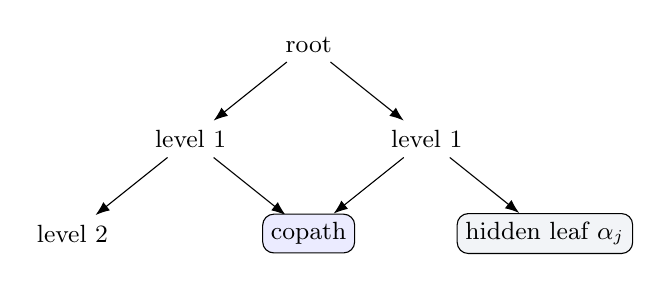
\begin{tikzpicture}[
  level distance=12mm,
  sibling distance=30mm,
  every node/.style={font=\small},
  edge from parent/.style={draw, -{Latex[length=1.8mm]}},
  hidden/.style={draw, rounded corners, fill=vorb3gray, inner sep=3pt},
  copath/.style={draw, rounded corners, fill=blue!8, inner sep=3pt}
]
\node {root}
  child {node {level 1}
    child {node {level 2}}
    child {node {level 2}}}
  child {node {level 1}
    child {node[copath] {copath}}
    child {node[hidden] {hidden leaf $\alpha_j$}}};
\end{tikzpicture}
\caption{GGM/Merkle tree with one hidden leaf and the copath. The verifier
re-expands the sibling subtree, recomputes the hidden commitment from the
signature, and combines bottom-up to the root.}
\label{fig:ggm}
\end{figure}

\subsection{Root reconstruction}

The verifier starts with $\com_{j,\alpha_j}$ at level 8 and the copath. For
each level from 8 down to 1:
\begin{enumerate}
  \item the sibling seed expands to its subtree; its leaf commitments and
        internal hashes produce the sibling node hash at that level;
  \item if the current node is a left child, the parent is
        $\WH(\ldots\concat\mathsf{current}\concat\mathsf{sibling})$;
        otherwise the order is reversed;
  \item the result becomes the current node for the next level.
\end{enumerate}
The final level-0 hash must equal the root absorbed into the transcript.
The verifier MUST NOT re-expand the hidden subtree; the hidden commitment is
bound by the root.

\section{VOLE correlation and wire assignment}

\subsection{Correlation}

For a hidden leaf:
\[
u=\text{prover share},\qquad
q=\mathsf{field}(\com[0:\Fbytes]),\qquad
v=q\xor u\delta.
\]
After the prover sends $d=u\xor w$:
\[
q'=q\xor d\delta=v\xor w\delta.
\]
The verifier knows $q,d,\delta,q'$; the prover knows $u,v,w$. The value $w$ is
one-time-padded by $u$.

\subsection{Wire map}

\begin{table}[ht]
\centering
\small
\caption{Wire map (same indices in every profile).}
\label{tab:wiremap}
\begin{tabular}{@{}cll@{}}
\toprule
Index & Tree & Meaning \\
\midrule
0 & 0 & $\sk$ \\
1--15 & 1--15 & $y_0,\ldots,y_{14}$ \\
16--30 & 16--30 & $b_0,\ldots,b_{14}$ \\
-- & 31 & mask $(u^\ast,v^\ast)$ \\
\bottomrule
\end{tabular}
\end{table}

\subsection{Linear wires}

The initial and linear wires are:
\begin{align}
\pt &: w=\pt, && q=\pt\delta, && v=0,\\
0 &: w=0, && q=0, && v=0,\\
1 &: w=1, && q=\delta, && v=0,\\
K_r &: w=K_r, && q=K_r\delta, && v=0,\\
x_r &: w=s_{r-1}\xor\sk\xor K_r, && q=q_s\xor q_{\sk}\xor K_r\delta, && v=v_s\xor v_{\sk},\\
s_r &: w=c_r y_r, && q=c_r q_{y_r}, && v=c_r v_{y_r},\\
1\xor b_r &: w=1\xor b_r, && q=\delta\xor q_{b_r}, && v=v_{b_r}.
\end{align}
The final ciphertext is $\ct=s_{14}\xor\sk$, with
$q_{\ct}=q_s\xor q_{\sk}$ and $v_{\ct}=v_s\xor v_{\sk}$. The prover sends
$\outtag=v_{\ct}$; the verifier checks
$q_{\ct}=\outtag\xor\ct\delta$.

\section{QuickSilver proof}

\subsection{Gate equations}

For each round $r$, the four gates are:
\begin{align}
&(b_r,b_r,b_r),\\
&(b_r,x_r,0),\\
&(b_r,y_r,0),\\
&(x_r,y_r,1\xor b_r).
\end{align}
For a gate $(a,b,c)$ the prover computes
\[
A_{0,i}=v_a v_b,\qquad
A_{1,i}=w_a v_b\xor w_b v_a\xor v_c.
\]
The verifier computes
\[
B_i=q_a q_b\xor q_c\delta.
\]

\subsection{Batching}

Let $\chi$ be the transcript challenge and $G=60$. The prover computes
\[
A_0=\bigoplus_{i=0}^{G-1}A_{0,i}\chi^i,\qquad
A_1=\bigoplus_{i=0}^{G-1}A_{1,i}\chi^i,
\]
and the verifier computes
\[
B=\bigoplus_{i=0}^{G-1}B_i\chi^i.
\]

\subsection{Mask}

With the mask tree $31$ and $q^\ast=\com_{31}[0:\Fbytes]$,
\[
v^\ast=q^\ast\xor u^\ast\delta,\qquad
U=A_0\xor v^\ast,\qquad
V=A_1\xor u^\ast.
\]
The verifier checks
\[
B\xor q^\ast=U\xor V\delta.
\]
The values $u^\ast,v^\ast$ are a one-time pad; the verifier knows only
$q^\ast$.

\subsection{Soundness condition}

For an incorrect multiplication gate, the difference
$B_i\xor A_{0,i}\xor A_{1,i}\delta$ is a nonzero polynomial in $\delta$ of
degree at most two. A random $\delta$ therefore detects a wrong gate with
probability at least $1-2/|\F{b}|$. The batched check uses a random $\chi$;
the conservative union bound over $G$ gates is $2G/|\F{b}|$. This is the
accounting used in the security case.

\section{Key generation}

\begin{algorithm}[ht]
\caption{$\Gen(\mathsf{seed})$}
\label{alg:keygen}
\begin{algorithmic}[1]
\REQUIRE seed $s\in\{0,1\}^{\Fbytes}$
\ENSURE $(\sk,\pt,\ct,\pk)$
\STATE $\sk\gets\mathsf{nonzero}(\mathsf{field}(\KDF_\Fbytes(\texttt{VORB3-KEYGEN-SK-V1},s)))$
\STATE $\pt\gets\mathsf{nonzero}(\mathsf{field}(\KDF_\Fbytes(\texttt{VORB3-KEYGEN-PT-V1},s)))$
\STATE $\ct\gets\Rain(\sk,\pt)$
\STATE reject if $\sk=0$ or $\pt=0$ or $\ct=0$
\STATE $\pk\gets\mathsf{bytes}(\pt)\concat\mathsf{bytes}(\ct)$
\RETURN $(\sk,\pt,\ct,\pk)$
\end{algorithmic}
\end{algorithm}

The expanded secret is $\mathsf{bytes}(\sk)\concat\mathsf{bytes}(\pt)
\concat s$ and is zeroized on drop. The public key is exactly $2\Fbytes$ bytes.

\section{Signing}

\subsection{Inputs and preprocessing}

Inputs: message $m$ (arbitrary length), expanded secret
$(\sk,\pt,\mathsf{seed})$, entropy $e\in\{0,1\}^{256}$. Signing proceeds as
follows.

\begin{enumerate}
  \item Validate $\sk\ne0$, $\pt\ne0$; compute $\ct=\Rain(\sk,\pt)$ and reject
        if $\ct=0$.
  \item $\pk=\mathsf{bytes}(\pt)\concat\mathsf{bytes}(\ct)$.
  \item $\mathsf{pkh}=\WH(\texttt{VORB3-PK-HASH-V1}\concat\pk)$.
  \item $\master=\KDF_\Fbytes(\texttt{VORB3-HEDGED-V1},
        \mathsf{bytes}(\sk)\concat\pk\concat\mathsf{u64le}(|m|)\concat m\concat e)$.
  \item $\salt=\WH(\texttt{VORB3-SALT-V1}\concat\master)$.
\end{enumerate}

\subsection{Pass A: roots}

For $j=0,\ldots,\Trees-1$:
\begin{enumerate}
  \item derive $\mathsf{root\_seed}_j$;
  \item expand the full GGM tree;
  \item compute leaf shares and commitments;
  \item compute internal node hashes and the root.
\end{enumerate}
Store the $\Trees$ roots as $\mathsf{roots}=r_0\concat\cdots\concat r_{\Trees-1}$.

\subsection{Transcript and challenges}

Absorb $\texttt{PK}$, $\texttt{SALT}$, $\texttt{MSG}$, and $\texttt{ROOTS}$.
Squeeze:
\[
\delta=\mathsf{nonzero}(\mathsf{field}(\mathsf{squeeze}(\texttt{DELTA},32))),
\quad
\chi=\mathsf{nonzero}(\mathsf{field}(\mathsf{squeeze}(\texttt{CHI},32))),
\]
and $\htwo=\mathsf{squeeze}(\texttt{H2},64)$. Set
$\alpha_j=\htwo[j]$ for $j=0,\ldots,\Trees-1$.

\subsection{Pass B: openings}

For $j=0,\ldots,\Trees-1$:
\begin{enumerate}
  \item re-expand tree $j$;
  \item extract the copath for $\alpha_j$;
  \item compute the hidden leaf share $u_j$ and commitment $\com_j$;
  \item set $q_j=\mathsf{field}(\com_j[0:\Fbytes])$.
\end{enumerate}
The mask tree is $j=31$; trees $32$--$34$ (default only) are committed but
unused by wires.

\subsection{Rain witness and wires}

Compute $(x_r,y_r,b_r,s_r)$ and $\ct$. Fill the 31 wires in the order of
Table~\ref{tab:wiremap}. For each wire $i$:
\[
d_i=u_i\xor w_i,\qquad
q_i'=q_i\xor d_i\delta,\qquad
v_i=q_i\xor u_i\delta.
\]
A debug build checks $q_i'=v_i\xor w_i\delta$.

\subsection{Proof assembly}

Compute the 60 gate pairs $(A_{0,i},A_{1,i})$, batch with $\chi$ to obtain
$A_0,A_1$, and compute
\[
U=A_0\xor v^\ast,\qquad V=A_1\xor u^\ast,
\]
where $(u^\ast,v^\ast)$ is the mask. Compute $\outtag=v_{\ct}$.

\subsection{Serialization and wipe}

Serialize in the order of Section~\ref{sec:serialization}. On every exit
path, wipe $\master$, tree seeds, leaf seeds, $u$, $v$, witness values, and
intermediate gate values. The signature contains only fixed-size fields and
no unbound padding.

\section{Verification}

\begin{algorithm}[ht]
\caption{$\Verify(\pk,m,\sigma)$}
\label{alg:verify}
\begin{algorithmic}[1]
\REQUIRE $\pk\in\{0,1\}^{2\Fbytes}$, $m$, $\sigma\in\{0,1\}^{\mathsf{SIG}}$
\ENSURE accept or uniform reject
\STATE reject if $|\sigma|\ne\mathsf{SIG}$
\STATE decode $\pt,\ct$; reject if either is zero
\STATE parse $\salt,\htwo,d,U,V,\outtag,\copath,\com$
\FOR{$j=0$ to $\Trees-1$}
  \STATE $\mathsf{root}_j\gets\mathsf{reconstruct}(\com_j,\copath_j)$
\ENDFOR
\STATE recompute transcript with $\pk,\salt,m,\mathsf{roots}$
\STATE squeeze $(\delta',\chi',\htwo')$; check $\htwo'=\htwo$ in constant time
\STATE map zero $\delta',\chi'$ to one
\FOR{$i=0$ to $30$}
  \STATE $q_i'\gets q_i\xor d_i\delta'$
\ENDFOR
\STATE compute $q$ for linear wires; compute $B_i$ for all gates
\STATE $B\gets\bigoplus_i B_i\chi'^i$
\STATE check $B\xor q^\ast=U\xor V\delta'$
\STATE check $q_{\ct}=\outtag\xor\ct\delta'$
\IF{all checks pass}
  \RETURN accept
\ELSE
  \RETURN reject
\ENDIF
\end{algorithmic}
\end{algorithm}

All signature-content failures return the same error. The verifier MUST NOT
take a secret-dependent early exit. Public-key validity is checked separately
from signature validity.

\section{Serialization}
\label{sec:serialization}

\subsection{Field encoding}

Field elements are $\Fbytes$ little-endian bytes. Hashes and roots are raw
64-byte strings. Seeds are $\Fbytes$ bytes. All lengths are fixed; there are
no variable-length fields and no trailing bytes.

\subsection{Layout}

\begin{table}[ht]
\centering
\small
\caption{Normative signature layout. Offsets are bytes.}
\label{tab:layout}
\begin{tabular}{@{}lrrr@{}}
\toprule
Field & SP-288/35 & Level 1+ & Level 3+ \\
\midrule
$\salt$ (offset 0) & 64 & 64 & 64 \\
$\htwo$ (offset 64) & 64 & 64 & 64 \\
$\mathsf{wire\_d}$ (offset 128) & 1,116 & 620 & 868 \\
$U$ & 36 & 20 & 28 \\
$V$ & 36 & 20 & 28 \\
$\outtag$ & 36 & 20 & 28 \\
$\copath$ & 10,080 & 5,120 & 7,168 \\
$\mathsf{hidden\_coms}$ & 2,240 & 2,048 & 2,048 \\
\midrule
Total & 13,672 & 7,976 & 10,296 \\
\bottomrule
\end{tabular}
\end{table}

The exact offsets are:
\begin{itemize}
  \item SP-288/35: $\salt[0:64]$, $\htwo[64:128]$, $\mathsf{wire\_d}[128:1244]$,
        $U[1244:1280]$, $V[1280:1316]$, $\outtag[1316:1352]$,
        $\copath[1352:11432]$, $\mathsf{hidden\_coms}[11432:13672]$;
  \item Level 1+: $\mathsf{wire\_d}[128:748]$, $U[748:768]$, $V[768:788]$,
        $\outtag[788:808]$, $\copath[808:5928]$,
        $\mathsf{hidden\_coms}[5928:7976]$;
  \item Level 3+: $\mathsf{wire\_d}[128:996]$, $U[996:1024]$, $V[1024:1052]$,
        $\outtag[1052:1080]$, $\copath[1080:8248]$,
        $\mathsf{hidden\_coms}[8248:10296]$.
\end{itemize}

\subsection{Ordering rules}

\begin{itemize}
  \item $\mathsf{wire\_d}$ is 31 field elements in wire order 0--30.
  \item Copaths are tree 0 to $\Trees-1$; within a tree, level 8 sibling first,
        then level 7 down to level 1.
  \item Hidden commitments are tree 0 to $\Trees-1$, each 64 bytes.
  \item The first $\Trees$ bytes of $\htwo$ are the hidden indices; the rest
        bind the transcript.
\end{itemize}

\section{Parsing and errors}

\subsection{Public key}

A public key is exactly $2\Fbytes$ bytes. It is rejected if either field
element is zero. There are no other validity checks.

\subsection{Signature}

A signature is exactly $\mathsf{SIG}$ bytes. Any other length is rejected.
There are no trailing bytes and no non-canonical field encodings.

\subsection{Error semantics}

\begin{table}[ht]
\centering
\small
\caption{API error mapping.}
\label{tab:errors}
\begin{tabular}{@{}ll@{}}
\toprule
Condition & Result \\
\midrule
Wrong signature length & \texttt{InvalidSignature} \\
Wrong public-key length & compile-time fixed; parse error \\
Zero $\pt$ or $\ct$ & \texttt{InvalidPublicKey} \\
Degenerate secret key & \texttt{InvalidSecretKey} \\
Transcript/$\htwo$ mismatch & \texttt{InvalidSignature} \\
Wire MAC mismatch & \texttt{InvalidSignature} \\
Gate/mask/output failure & \texttt{InvalidSignature} \\
\bottomrule
\end{tabular}
\end{table}

The implementation returns one uniform verification error for all
signature-content failures.

\section{Domain separation registry}

\begin{longtable}{@{}p{0.55\linewidth}p{0.38\linewidth}@{}}
\toprule
Label & Use \\
\midrule
\endhead
\texttt{VORB3-WH512-A-V1} & WH512 left \\
\texttt{VORB3-WH512-B-V1} & WH512 right \\
\texttt{VORB3-GGM-EXPAND-V1} & GGM expansion \\
\texttt{VORB3-KEYGEN-SK-V1} & secret key \\
\texttt{VORB3-KEYGEN-PT-V1} & plaintext \\
\texttt{VORB3-HEDGED-V1} & master seed \\
\texttt{VORB3-PK-HASH-V1} & public-key hash \\
\texttt{VORB3-TREE-ROOT-V1} & tree root seed \\
\texttt{VORB3-RAIN\{...\}-SP-CONST-V1} & Rain constants \\
\texttt{VORB3-RAIN\{...\}-SP-K\{r\}-V1} & Rain round keys \\
\texttt{VORB3-RAIN\{...\}-SP-C\{r\}-V1} & Rain diffusion constants \\
\texttt{VORB3-SALT-V1} & salt \\
\texttt{VORB3-GGM-LEAF-V1} & leaf commitment \\
\texttt{VORB3-GGM-NODE-V1} & internal node \\
\texttt{VORB3-TRANSCRIPT-INIT-V1} & transcript init \\
\texttt{VORB3-TRANSCRIPT-ABSORB-V1} & transcript absorb \\
\texttt{VORB3-TRANSCRIPT-SQUEEZE-V1} & transcript squeeze \\
\texttt{VORB3-TRANSCRIPT-RATCHET-V1} & transcript ratchet \\
\texttt{PK, SALT, MSG, ROOTS, DELTA, CHI, H2} & transcript labels \\
\bottomrule
\end{longtable}

Labels MUST NOT be reused with different parameters. Changing a label is a
protocol-version change.

\section{Test vectors}

\subsection{KAT files}

\begin{table}[ht]
\centering
\small
\caption{Frozen KAT files and signature digests.}
\label{tab:katfiles}
\begin{tabular}{@{}lccc@{}}
\toprule
Profile & Seed file & Public key file & Signature file \\
\midrule
SP-288/35 & \texttt{seed\_sp288\_35.bin} & \texttt{pk\_sp288\_35.bin} & \texttt{sign\_sp288\_35.bin} \\
Level 1+ & \texttt{seed\_sp160\_32.bin} & \texttt{pk\_sp160\_32.bin} & \texttt{sign\_sp160\_32.bin} \\
Level 3+ & \texttt{seed\_sp224\_32.bin} & \texttt{pk\_sp224\_32.bin} & \texttt{sign\_sp224\_32.bin} \\
\bottomrule
\end{tabular}
\end{table}

\begin{table}[ht]
\centering
\small
\caption{SHA-256 digests of the KAT files.}
\label{tab:kathashes}
\begin{tabular}{@{}lccc@{}}
\toprule
Profile & Seed & Public key & Signature \\
\midrule
SP-288/35 & \texttt{dd1b0529...} & \texttt{a7b5a252...} & \texttt{c073c7e3...} \\
Level 1+ & \texttt{88b90539...} & \texttt{7a0756e5...} & \texttt{43dcf2de...} \\
Level 3+ & \texttt{4248e3fd...} & \texttt{753312d0...} & \texttt{3ad501e1...} \\
\bottomrule
\end{tabular}
\end{table}

\subsection{Raw seed and public-key vectors}

\begin{align*}
\text{SP-288/35 seed} &= \texttt{46bc6ad6e6af38f0d15f3f1b56d8e28279cd735231de2a1ca0}\\
&\quad\texttt{abb8dc122d961f4b415421},\\
\text{SP-288/35 pk} &= \texttt{6380aa2da51f709e300b6a9f004c379007e9ebdc5aa7f592}\\
&\quad\texttt{69974a2045e64081cc761907b77d6c2570342e2e84f7d266}\\
&\quad\texttt{6ce9870c1b7e9491582882e8af91f255239047395cdb91b7},\\
\text{Level 1+ seed} &= \texttt{1e4fae52c4eb017ceb51cb1d365d8db45c7d8c79},\\
\text{Level 1+ pk} &= \texttt{ae858e22a60dbfbf7fdad02e5a33f38d6dad9ca2d568}\\
&\quad\texttt{2aab74367bd2b2cdf059aa8cfdaafb1bcf7d},\\
\text{Level 3+ seed} &= \texttt{3da55abb2a69d2ff59d0d33955d46c3c}\\
&\quad\texttt{b4cb28d347a88ede82442e5e},\\
\text{Level 3+ pk} &= \texttt{47218a679b90ff913cf7b6a0891d330494c998a5b1e8634}\\
&\quad\texttt{4d5947b63f5e27fedfa24ecf2a279396f01fd4e83324f0d12f}\\
&\quad\texttt{2842aabadc812319}.
\end{align*}

\subsection{Differential vectors}

\begin{itemize}
  \item Signature differential: 28 messages spanning 0--8192 bytes,
        including the boundary lengths $0,1,31,32,33,63,64,65,\ldots,
        8191,8192$; each record contains seed, public key, entropy, message,
        and signature.
  \item Field differential: 4,096 records for each compact field; each record
        contains two field elements, their product, and the inverse of the
        first.
\end{itemize}

\section{Constant-time and zeroization requirements}

\subsection{Control flow}

\begin{itemize}
  \item All secret-dependent operations MUST use fixed iteration counts.
  \item Secret values MUST NOT be used as array indices, loop bounds, or
        branch conditions.
  \item Selection of secret values MUST use mask-based constant-time
        selection.
  \item The verifier MUST accumulate checks and MUST NOT early-exit on
        signature-content failures.
  \item Compiler barriers (\texttt{black\_box}) MUST prevent the optimizer from
        introducing secret-dependent branches or eliminating wipes.
\end{itemize}

\subsection{Zeroization}

\begin{itemize}
  \item Owned secret buffers (secret key, expanded secret, master seed, tree
        seeds, leaf seeds, witness, openings, tags, masked values) SHOULD be
        wiped on every exit path.
  \item \texttt{Drop} implementations MUST wipe owned secret fields.
  \item Zeroization of compiler temporaries and registers is best-effort;
        the limitation is documented.
\end{itemize}

\subsection{Stack}

The library targets an internal working set of 32 KiB in release builds. A
caller that places the full signature on the stack MUST budget the larger
case: 64 KiB for the default profile, and the correspondingly smaller compact
signature sizes. The stack target is tested on the supported cross-runtime
matrix.

\section{API contract}

\begin{lstlisting}
pub const FIELD_BITS: usize;
pub const FIELD_BYTES: usize;
pub const PUBLIC_KEY_LEN: usize;
pub const SIGNATURE_LEN: usize;
pub const TREE_COUNT: usize;
pub const SPEC_VERSION: &str;

pub struct SecretKey;
pub struct ExpandedSecretKey;
pub struct PublicKey;
pub struct Signature;

impl SecretKey { pub const fn from_seed(seed: [u8; FIELD_BYTES]) -> Self; }
impl ExpandedSecretKey {
    pub fn from_seed(seed: &SecretKey) -> Self;
    pub fn public_key(&self) -> Result<PublicKey, Error>;
}
impl PublicKey {
    pub fn from_bytes(bytes: [u8; PUBLIC_KEY_LEN]) -> Result<Self, Error>;
}
impl Signature {
    pub fn from_bytes(input: &[u8]) -> Result<Self, Error>;
}

pub fn sign(message: &[u8], secret: &ExpandedSecretKey,
            entropy: &[u8; 32]) -> Result<Signature, Error>;
pub fn sign_into(message: &[u8], secret: &ExpandedSecretKey,
                 entropy: &[u8; 32],
                 signature: &mut [u8; SIGNATURE_LEN]) -> Result<(), Error>;
pub fn verify(message: &[u8], public: &PublicKey,
              signature: &Signature) -> Result<(), Error>;
pub fn verify_bytes(message: &[u8], public: &PublicKey,
                    signature: &[u8; SIGNATURE_LEN]) -> Result<(), Error>;
\end{lstlisting}

The caller is responsible for seed storage and entropy acquisition. The
all-zero entropy value is a test/KAT input, not a production RNG.

\section{Validation checklist}

A conforming implementation SHOULD pass the following checks:

\begin{enumerate}
  \item selected profile and feature exclusivity;
  \item frozen KAT (seed, public key, signature);
  \item signature and field differentials;
  \item single-bit signature sweep;
  \item wrong length, truncation, trailing-byte, and non-canonical parsing;
  \item wrong key, wrong message, replay, cross-context, swap, and duplication
        rejection;
  \item transcript and $\htwo$ binding;
  \item wire MAC, gate, mask, and output-tag checks;
  \item 32 KiB stack target in release;
  \item cross-runtime KATs on the supported matrix;
  \item reproducible build;
  \item zeroization and canary checks;
  \item mutation/fuzz/coverage gates recorded in the evidence set.
\end{enumerate}

\section{Security considerations}

The profile floors are conservative accounting targets:
SP-288/35 $\approx$140/256, Level 1+ $\approx$76.5/153.1, Level 3+
$\approx$108.5/217.1 (quantum/classical). The 256-bit field is not used for a
128-bit claim. The field-check term uses the conservative $2G/|\F{b}|$ union
bound. WH512 is assumed to have the generic 512-bit collision bound under
independent BLAKE3-domain instances.

The following are explicitly not claimed:
\begin{itemize}
  \item an external audit or NIST certification;
  \item a formal proof of Rain-SP1 security;
  \item a machine-checked soundness/ZK proof for the exact circuit;
  \item full symbolic Kani verification of sign/verify;
  \item a formal constant-time theorem;
  \item a 72-hour fuzz soak;
  \item hardware power/EM side-channel resistance.
\end{itemize}

Implementers MUST treat this document as a specification of a candidate
scheme, not as a security certificate.

\appendix

\section{Gate table}

\begin{longtable}{@{}clll@{}}
\toprule
\# & Equation & Prover values & Verifier value \\
\midrule
\endhead
$4r+1$ & $b_r^2=b_r$ & $v_bv_b$ & $q_bq_b\xor q_b\delta$ \\
$4r+2$ & $b_rx_r=0$ & $v_bv_x$ & $q_bq_x$ \\
$4r+3$ & $b_ry_r=0$ & $v_bv_y$ & $q_bq_y$ \\
$4r+4$ & $x_ry_r=1\xor b_r$ & $v_xv_y\xor v_{1\xor b}$ & $q_xq_y\xor q_{1\xor b}\delta$ \\
\bottomrule
\end{longtable}

The verifier's gate value is
$B_i=q_aq_b\xor q_c\delta$; the prover's pair is
$(A_{0,i},A_{1,i})=(v_av_b,\;w_av_b\xor w_bv_a\xor v_c)$.

\section{Formulas}

\begin{align}
\mathsf{SIG}&=128+34\Fbytes+\Trees(8\Fbytes+64),\\
\pk&=2\Fbytes,\qquad \sk_{\mathrm{compact}}=\Fbytes,\qquad
\sk_{\mathrm{expanded}}=3\Fbytes,\\
\ct&=s_{14}\xor\sk,\\
q'&=q\xor d\delta=v\xor w\delta,\\
B&=\bigoplus_{i=0}^{59}B_i\chi^i,\\
U&=A_0\xor v^\ast,\qquad V=A_1\xor u^\ast.
\end{align}

\section{Implementation notes}

The compact field uses 32-bit limbs, bit-interleaved squaring, word-level
reduction, and an Itoh--Tsujii inversion chain. The v1.3.0 measurements are:
Level 1+ multiplication 216 ns, squaring 10.5 ns, inversion 4.43 $\mu$s;
Level 3+ 409 ns, 11.8 ns, 9.40 $\mu$s. The default 288-bit field uses 64-bit
limbs with a specialized square and a 16-entry Itoh--Tsujii chain. The
implementation is fixed-iteration and branches only on public parameters.

\section{Release and evidence manifest}

\begin{table}[ht]
\centering
\small
\caption{Release-line summary. See \texttt{docs/RELEASES.md} for the full
evidence and hashes.}
\label{tab:releases}
\begin{tabular}{@{}lll@{}}
\toprule
Tag & Profile & Summary \\
\midrule
v1.0.0 & SP-288/35 & frozen default release \\
v1.1.0 & Level 1+ & compact pack introduction \\
v1.2.0 & Level 3+ & compact pack introduction \\
v1.3.0 & both compact packs & field optimization + full benchmarks \\
\bottomrule
\end{tabular}
\end{table}

\begin{thebibliography}{9}
\bibitem{GGM86}
O. Goldreich, S. Goldwasser, and S. Micali.
\newblock How to construct random functions.
\newblock \emph{Journal of the ACM}, 33(4):792--807, 1986.

\bibitem{Merkle87}
R. C. Merkle.
\newblock A digital signature based on a conventional encryption function.
\newblock In \emph{CRYPTO}, 1987.

\bibitem{FS86}
A. Fiat and A. Shamir.
\newblock How to prove yourself: Practical solutions to identification and
signature problems.
\newblock In \emph{CRYPTO}, 1986.

\bibitem{QuickSilver}
C. Baum, L. Braun, C. Delpech de Saint Guilhem, M. Kloo\ss,
E. Orsini, L. Roy, and P. Scholl.
\newblock QuickSilver: Efficient and affordable zero-knowledge proofs for
circuits and polynomials over any field.
\newblock In \emph{ACM CCS}, 2021.

\bibitem{VOLEitH}
C. Baum, C. Delpech de Saint Guilhem, M. Kloo\ss, E. Orsini, and P. Scholl.
\newblock VOLEitH: Making VOLE-based zero-knowledge proofs transparent.
\newblock In \emph{CRYPTO}, 2022.

\bibitem{BLAKE3}
J. O'Connor, J.-P. Aumasson, S. Neves, and Z. Wilcox-O'Hearn.
\newblock BLAKE3: One function, fast everywhere.
\newblock 2020. \url{https://blake3.io}.

\end{thebibliography}

\end{document}
